\documentclass{beamer}
\usetheme{Frankfurt}
%\usecolortheme{seahorse}

\title{Advanced simulations}
\author
{Walter Van Herck\inst{1}}
\institute[JCNS at MLZ] % (optional)
{
  \inst{1}%
  J\"ulich Centre for Neutron Science at MLZ
}
\date[BornAgain] % (optional)
{BornAgain School and User Meeting, 2018}
\subject{Computer Science}

\begin{document}

\frame[plain]{\titlepage}

\begin{frame}
    \frametitle{Overview}
    \tableofcontents
\end{frame}

\section{Time resolved GISAS}

\begin{frame}
    \frametitle{Rotating square lattice movie}
        A sample with cylinders in a square lattice arrangement\
        is rotated during the measurement along the z-axis.
    \begin{figure}
        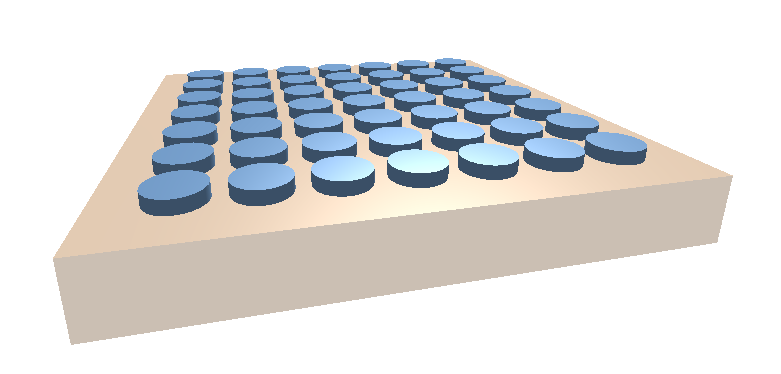
\includegraphics[width=8cm]{rotation_movie.png}
    \end{figure}
\end{frame}

\section{Deep learning with BornAgain}

\begin{frame}
    \frametitle{Deep learning with BornAgain}
    \begin{itemize}
        \item Motivation
        \item Neural networks and deep learning
        \item Data generation
        \item Training
        \item Validation
    \end{itemize}
\end{frame}

\begin{frame}
    \frametitle{Motivation}
    Hexagonally arranged $CoFe_2O_4$ nanoparticles.
    \begin{figure}
        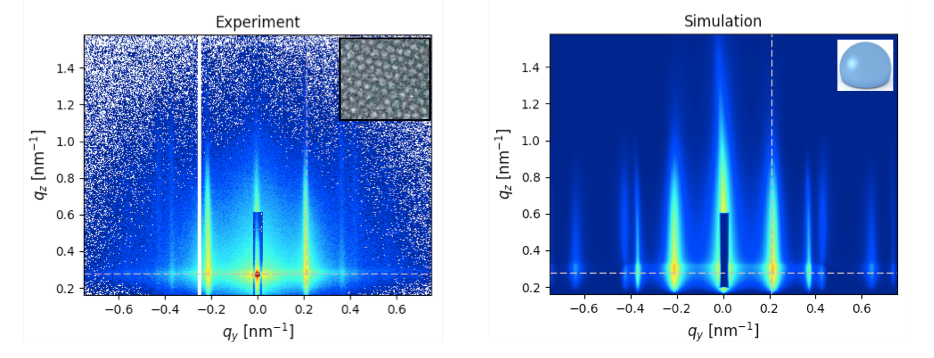
\includegraphics[width=10cm]{asma_ganeva.png}
        \\ \tiny{A. Qdemat, E. Kentzinger, G. Portale, M. Ganeva, U. Rücker,\
         Th. Brückel}
    \end{figure}
    Despite the good correspondence between data and simulation, it \
    is hard to state that all orientation information is captured by it.
\end{frame}

\begin{frame}
    \frametitle{Motivation}
    \begin{itemize}
        \item A 120 parameter fit is unfeasable.
        \item We investigate if deep learning might help analyzing this type\
              of complex data.
    \end{itemize}
    \begin{figure}
        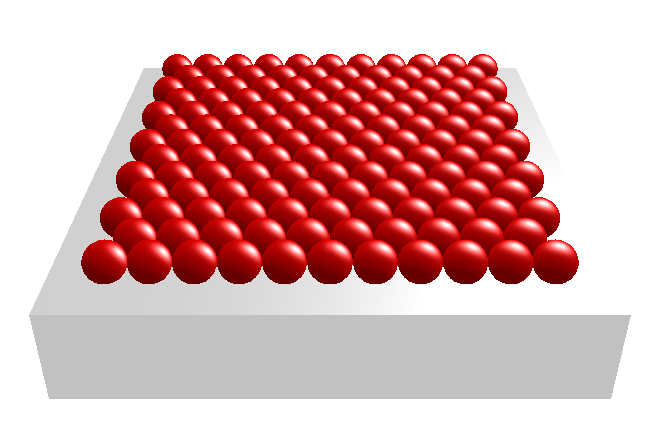
\includegraphics[width=5cm]{orient_1.png}
        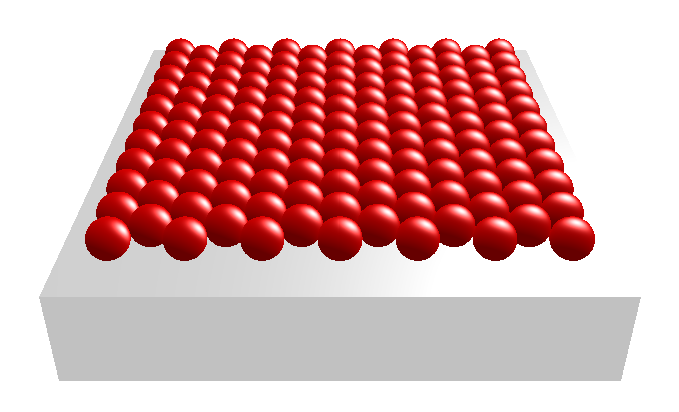
\includegraphics[width=5cm]{orient_2.png}
    \end{figure}
\end{frame}

\begin{frame}
    \frametitle{Neural networks}
    A neural network consists of a succession of layers that combine a linear
    mapping with some non-linear function.
    \begin{figure}
        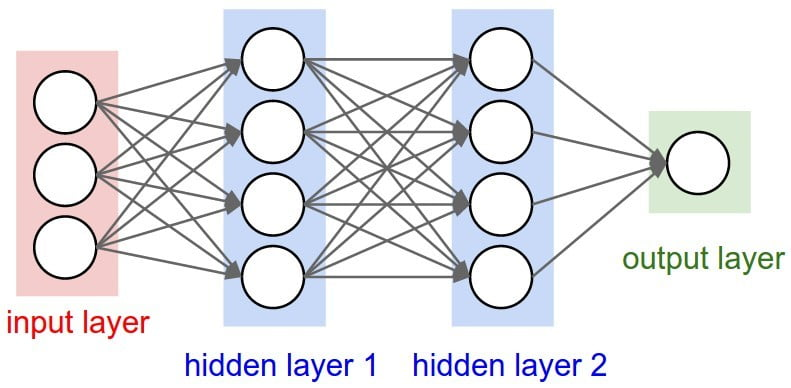
\includegraphics[width=10cm]{neural_network.jpg}
    \end{figure}
\end{frame}

\begin{frame}
    \frametitle{Data generation}
    Generate data for training/validation:
    \begin{itemize}
        \item Input: scattering image
        \item label: distribution of lattice orientations
        \item Using BornAgain python API
        \item 50k training, 10k validation examples
        \item Fixed: picture size, alignment, lattice lengths, peak shape
        \item Maximum 5 non-zero probabilities for \\
              angles in [0, 0.5, 1.0, ..., 60] degrees
        \item Input data shifted and rescaled to standard normal distribution
    \end{itemize}
\end{frame}

\begin{frame}
    \frametitle{Training}
    A neural network is trained by minimizing the \emph{difference} between\
    the predicted and the real distribution of lattice orientations.
    \begin{figure}
        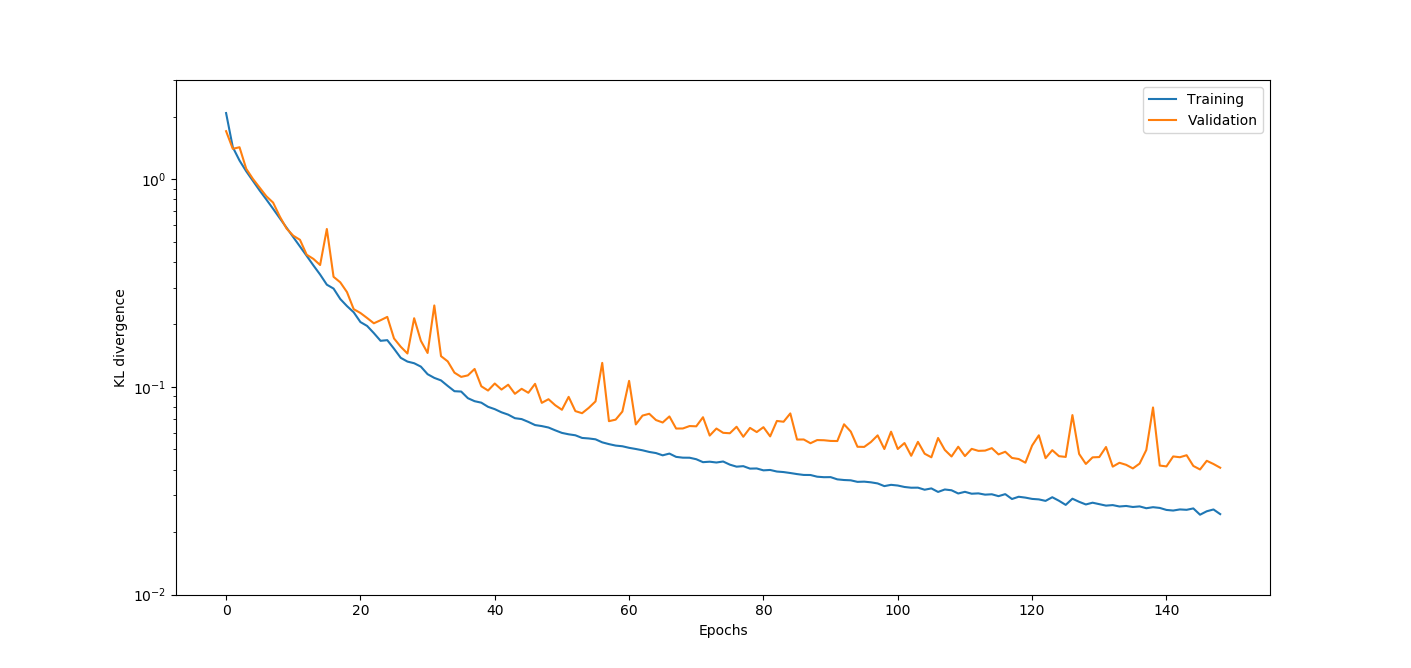
\includegraphics[width=10cm]{losses.png}
    \end{figure}
\end{frame}

\begin{frame}
    \frametitle{Validation}
    \begin{figure}
        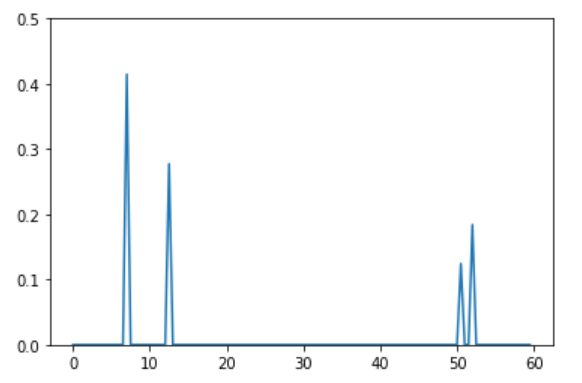
\includegraphics[width=4cm]{distr_orig.png}
        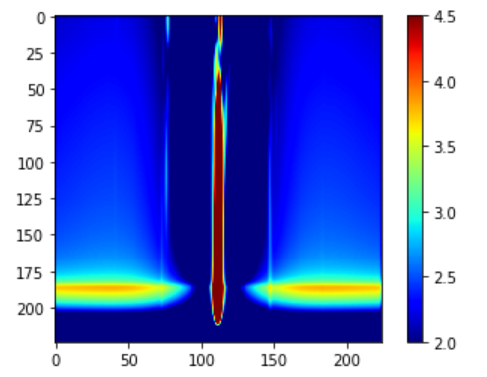
\includegraphics[width=4cm]{intensity_orig.png}
    \end{figure}
    \begin{figure}
        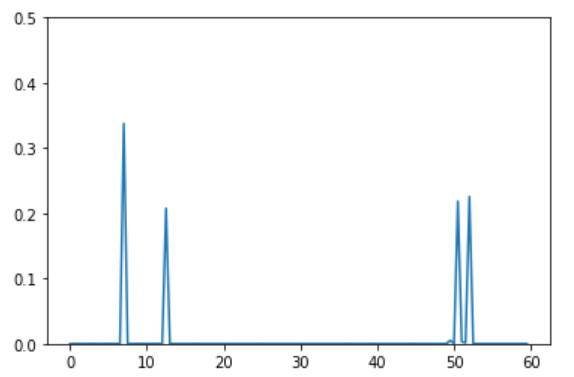
\includegraphics[width=4cm]{distr_pred.png}
    \end{figure}
\end{frame}

\end{document}